\chapter{Basic commands if the GIT} 
%pt
echo "# Articles" >> README.md
git init
git add README.md
git commit -m "first commit"
git branch -M main
git remote add origin https://github.com/FabioCamposFerreira/Articles.git
git push -u origin main
 \section{Gerando commit depois de modificar o projeto}
git status

%en
 This command 

%pt
 Este comando mostra o estado atual do seu projeto e o que deve ser feito para que ele esteja sincronizado e commitado. Ganhe o abto de executalo e lelo com atenção, para poder entender o que o git está fazendo.

git add <> 

%pt
 Use este comando para adicionar os 
git add .
%pt
 add. use este para adicionar todos os arquivos. Mas cuidado para não adicionar arquivos de cache pessados como o node. O git apresenta a função de ignorar arquivos com certas extenções justamente para você não ter que se preocupar com isso.
git pull

%en
 Update local repository with new changes in remote	 repository

%pt

git clone
%pt



git push

git commit -m ""

git fetch

%pt 
Realiza o download das mudanças comtidas no repositrio online. A diferença com o git pull é que o fetch não realiza a unificação das versões.

git remote

git checkout origin

git remote master

git config --global core.editor code

%pt 
Define o Visual Studio Code como editor padrão do git

%pt 
\section{Como remover todos os arquivos recursivamente?}
git reset HEAD -- *


\section{Resolvendo conflitos de versão}

git pull --rebase

%pt
quanto o git pull falha e gera a mensagem \textit{fatal: Not possible to fast-forward, aborting.}, significa que existem conflitos de commits entre o repositorio local e o remoto. Para resolver estes conflitos, use o comando acima e abra o edutor de texto padrão do git. Depois é so selecionar manualmente o que deseja resolver os conflitos
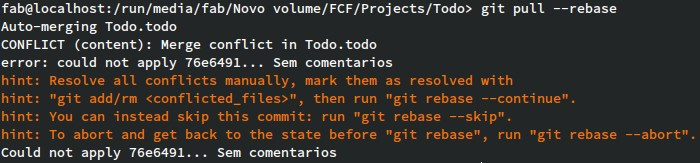
\includegraphics{img_erro_auto_mergeing.jpg}
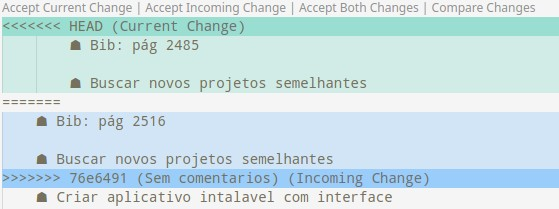
\includegraphics{img_erro_auto_mergeing_editor.jpg}

git rebase --continue

pt Use este ocmando para ir e resolver o próximo conflito

pt Quando não existir mais conflitos os conflitos, sinta-se livre para realizar o git push

pt \section{Boas praticas}

pt Considerar os commits como documentação

pt Escrever o que foi feito, o que não foi feito e porque 

pt Usar título A primeira linha de um commit serve como título

pt Fazer vários commits, porém fazer o rebase Uma das funções do git é servir de backup remoto. Você pode fazer commits diretos com as tentativas de arrumar um problema, ou mesmo fazer commits todos os dias. Na hora do PR, é só juntar as alterações feitas, descartar o lixo e fazer um ou mais commits relevantes. O mesmo serve para a revisão de código de um PR. Basta ir fazendo as alterações necessárias e depois fazer um rebase para unir tudo com o commit principal. Isso gera uma árvore limpa e fácil de navegar. 

pt Manter o repositório local atualizado (de preferência com rebase) É só ficar fazendo git fetch --all e git rebase origin/<nome da branch principal> que você vai manter a sua árvore sempre atualizada e isso evita maiores dores de cabeça na hora de criar o PR.

pt Proteger a master Acidentes acontecem, por isso é importante impedir as pessoas de fazerem pushs direto na master ou develop. Isso é feito através da configuração do repositório.

pt Não comitar grandes arquivos binários O git funciona muito bem para arquivos de textos e pequenos binários (coisa de alguns KB). No momento que você começa a colocar arquivos maiores, começa o diretório .git começa a dar ruim (principalmente se você mexer muito nesse arquivo)

pt Usar um bom .gitignore Um bom .gitiginore ajuda a evitar o envio de arquivos binários. Eu Eu gosto bastante o do gitiginore.io.

%en \chapter{References}]
Playlist
https://www.youtube.com/playlist?list=PLbEOwbQR9lqzK14I7OOeREEIE4k6rjgIj
https://dev.to/lucasscharf/boas-praticas-para-usar-o-git-2e0e